%% Font size %%
\documentclass[11pt]{article}

%% Load the custom package
\usepackage{Mathdoc}

%% Numéro de séquence %% Titre de la séquence %%
\renewcommand{\centerhead}{S04 - Les angles}


\usetikzlibrary{calc}
% Croix sur un point
\newcommand{\croix}[1]{\draw #1 ++(-2pt,-2pt) -- ++(4pt,4pt) ++(-4pt,0) -- ++(4pt,-4pt);}
% Angle du tableau des angles particuliers : \angleTab{mesure}
% Sommet O, côté [OA) horizontal vers la droite, côté [OB) tourné de « mesure ».
\newcommand{\angleTab}[1]{%
  \begin{tikzpicture}[baseline=(O.base)]
    \coordinate (O) at (0,0);
    \ifnum#1=90 \draw[gray!70!black, fill=gray!25] (0,0) rectangle (3mm,3mm);
    \else\ifnum#1>0 \draw[gray!70!black, fill=gray!25] (0,0) -- (4mm,0) arc[start angle=0, delta angle=#1, radius=4mm] -- cycle;
    \fi\fi
    \draw[thick] (1.25,0) -- (0,0) -- (#1:1.25);
    \fill (0,0) circle (1.2pt);
    \node[below] at (0,0) {$O$};
    \croix{(1,0)} \node[below] at (1,0) {$A$};
    \ifnum#1=0 \croix{(0.6,0)} \node[above] at (0.6,0) {$B$};
    \else\ifnum#1=180 \croix{(-1,0)} \node[below] at (-1,0) {$B$};
    \else \croix{(#1:1)} \node at ($(#1:1)+({#1+90}:3mm)$) {$B$};
    \fi\fi
  \end{tikzpicture}%
}
% Rapporteur dessiné (centre à l'origine, rayon 2.6) :
% graduation extérieure : 0 à droite ; graduation intérieure : 0 à gauche.
\newcommand{\rapporteur}{%
  \fill[blue!4] (3.3,0) arc[start angle=0, end angle=180, radius=3.3] -- cycle;
  \draw[blue!60!black] (3.3,0) arc[start angle=0, end angle=180, radius=3.3] -- cycle;
  \draw[blue!60!black] (2.1,0) arc[start angle=0, end angle=180, radius=2.1];
  \foreach \t in {0,5,...,180} \draw[blue!60!black] (\t:3.3) -- (\t:3.15);
  \foreach \t in {0,10,...,180} {
    \draw[blue!60!black] (\t:3.3) -- (\t:3.0);
    \node[blue!60!black, font=\fontsize{4.5pt}{5pt}\selectfont, inner sep=0pt, rotate=\t-90] at (\t:2.8) {\t};
    \pgfmathtruncatemacro{\u}{180-\t}
    \node[blue!60!black, font=\fontsize{4.5pt}{5pt}\selectfont, inner sep=0pt, rotate=\t-90] at (\t:2.45) {\u};
  }
  \draw[blue!60!black] (-0.15,0) -- (0.15,0) (0,0) -- (0,0.15);
}
% Encadré « compétence » en tête de partie
\newcommand{\comp}[2]{\par\smallskip\noindent\colorbox{gray!15}{\parbox{\dimexpr\linewidth-2\fboxsep}{\small\textbf{Compétence #1} : #2}}\par\smallskip}

%% Spacing commands %%
\renewcommand{\baselinestretch}{1} \setlength{\parindent}{0pt}

\begin{document}

\begin{tcolorbox}[colback=white,colframe=black,boxrule=0.6pt,arc=2mm,title={\textbf{Ce que je dois savoir faire à la fin du chapitre}},coltitle=black,colbacktitle=gray!15]
\begin{tabular}{@{}ll@{}}
\textbf{6C04-GEO10} & \textbf{Nommer} un angle \hfill (partie 1)\\
\textbf{6C04-GEO11} & Donner le \textbf{sommet} et les \textbf{côtés} d'un angle \hfill (partie 1)\\
\textbf{6C04-GEO12} & Reconnaître la \textbf{nature} d'un angle (nul, aigu, droit, obtus, plat) \hfill (partie 2)\\
\textbf{6C04-GEO13} & \textbf{Classer} des angles selon leur nature \hfill (partie 2)\\
\textbf{6C04-GEO14} & \textbf{Mesurer} un angle au rapporteur \hfill (partie 3)\\
\textbf{6C04-GEO15/16} & \textbf{Construire} un angle de mesure donnée \hfill (partie 4)\\
\end{tabular}
\end{tcolorbox}

\section{Vocabulaire : nommer un angle}

\begin{definition}
Deux \textbf{demi-droites de même origine} forment un \textbf{angle}.
\end{definition}

\subsection{Sommet et côtés}
\comp{6C04-GEO11}{donner le sommet et les côtés d'un angle \hfill \textit{Fiche Ex-6C04-02}}

\begin{vocabulaire}
\begin{itemize}
\item L'origine commune des deux demi-droites est le \textbf{sommet} de l'angle (c'est un \textbf{point}).
\item Les deux demi-droites sont les \textbf{côtés} de l'angle. Elles commencent au sommet :
on écrit le sommet \textbf{en premier}, avec un crochet : $[BA)$, $[BC)$.
\end{itemize}
\end{vocabulaire}

\begin{center}
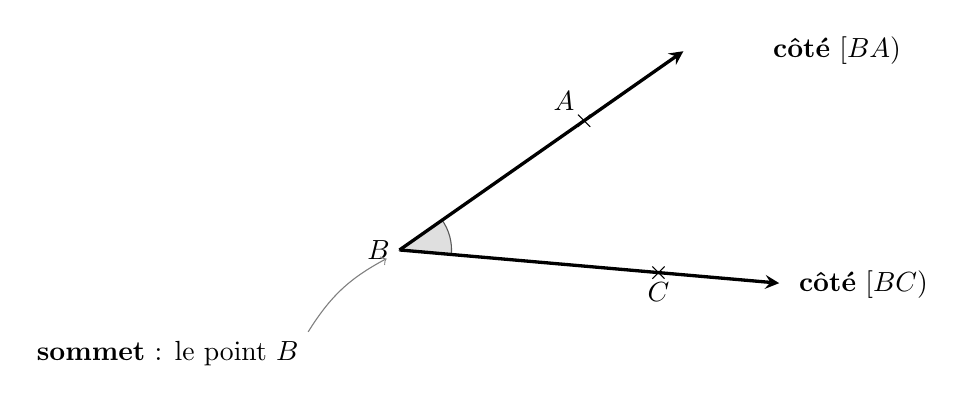
\begin{tikzpicture}[scale=1.1]
  \coordinate (B) at (0,0); \coordinate (A) at (35:2.6); \coordinate (C) at (-5:3);
  \draw[gray!70!black, fill=gray!25] (B) -- (-5:6mm) arc[start angle=-5, delta angle=40, radius=6mm] -- cycle;
  \draw[very thick,->,>=stealth] (B) -- (35:4);
  \draw[very thick,->,>=stealth] (B) -- (-5:4.4);
  \foreach \P in {A,C} \draw (\P) ++(-2pt,-2pt) -- ++(4pt,4pt) ++(-4pt,0) -- ++(4pt,-4pt);
  \node[above left] at (A) {$A$}; \node[below] at (C) {$C$}; \node[left] at (B) {$B$};
  \node[anchor=west,align=left] (s) at (-4.3,-1.2) {\textbf{sommet} : le point $B$};
  \draw[->,gray] (s.north east) to[bend left=15] (-0.15,-0.1);
  \node[anchor=west,align=left] at (4.2,2.3) {\textbf{côté} $[BA)$};
  \node[anchor=west,align=left] at (4.5,-0.4) {\textbf{côté} $[BC)$};
\end{tikzpicture}
\end{center}

\subsection{Nommer un angle}
\comp{6C04-GEO10}{nommer un angle avec trois lettres \hfill \textit{Fiche Ex-6C04-01}}

\begin{notation}
Pour nommer un angle, on écrit \textbf{trois lettres} sous un \textbf{chapeau} : $\widehat{ABC}$.
\begin{itemize}
\item la lettre \textbf{du milieu} est \textbf{le sommet} ;
\item les deux autres lettres sont des points, \textbf{un sur chaque côté}.
\end{itemize}
\end{notation}

\begin{exemple}
L'angle de la figure ci-dessus se note $\widehat{ABC}$ ou $\widehat{CBA}$ (même angle : le sommet $B$ reste au milieu).\\
Son sommet est le point $B$, ses côtés sont les demi-droites $[BA)$ et $[BC)$.
\end{exemple}

\begin{remarque}
\textbf{Attention :} $\widehat{BAC}$ n'est \textbf{pas} le même angle : son sommet est $A$ ! \\
Si plusieurs points sont sur un même côté, l'angle a plusieurs noms : si $D \in [BA)$, alors $\widehat{ABC} = \widehat{DBC}$.
\end{remarque}

\section{Nature d'un angle : les angles particuliers}
\comp{6C04-GEO12 et GEO13}{reconnaître la nature d'un angle, classer des angles \hfill \textit{Fiches Ex-6C04-03 et 04}}

\begin{definition}
Il y a \textbf{cinq} angles particuliers à connaître : l'angle \textbf{nul}, l'angle \textbf{aigu}, l'angle \textbf{droit},
l'angle \textbf{obtus} et l'angle \textbf{plat}. Pour trouver la nature d'un angle, on le compare à l'\textbf{angle droit}
(codé par un petit carré) et à l'\textbf{angle plat}.
\end{definition}

\begin{center}
\renewcommand{\arraystretch}{1.3}
\begin{tabularx}{\linewidth}{|>{\centering\arraybackslash}m{1.9cm}|*{5}{>{\centering\arraybackslash}X|}}
\hline
\textit{Nom} & \textbf{Angle nul} & \textbf{Angle aigu} & \textbf{Angle droit} & \textbf{Angle obtus} & \textbf{Angle plat} \\ \hline
\textit{Figure} &
\rule{0pt}{1.6cm}\angleTab{0} &
\angleTab{40} &
\angleTab{90} &
\angleTab{135} &
\angleTab{180} \\[3mm] \hline
\textit{Je le reconnais} &
Les deux côtés sont confondus &
Plus \textbf{petit} qu'un angle droit &
Il est codé par un \textbf{petit carré} &
Plus \textbf{grand} qu'un angle droit, plus petit qu'un plat &
Les côtés sont dans le prolongement : $A$, $O$, $B$ \textbf{alignés} \\ \hline
\textit{Mesure} & $0\degre$ & entre $0\degre$ et $90\degre$ & $90\degre$ & entre $90\degre$ et $180\degre$ & $180\degre$ \\ \hline
\end{tabularx}
\end{center}

\begin{remarque}
Un angle droit, c'est la \textbf{moitié} d'un angle plat : $180\degre \div 2 = 90\degre$.
\end{remarque}

\begin{exercice}[0][Exercice traité : reconnaître et classer]
\textbf{Méthode :} je compare l'angle à un angle droit.
\begin{itemize}
\item Les deux côtés sont \textbf{confondus} $\to$ l'angle est \textbf{nul}.
\item Il est \textbf{plus petit} qu'un angle droit $\to$ \textbf{aigu} ;\quad codé par un \textbf{petit carré} $\to$ \textbf{droit}.
\item Il est \textbf{plus grand} qu'un angle droit $\to$ \textbf{obtus} ;\quad les points sont \textbf{alignés} $\to$ \textbf{plat}.
\end{itemize}
\textbf{Classer les mesures} $35\degre$ ; $90\degre$ ; $150\degre$ ; $180\degre$ ; $89\degre$ ; $91\degre$ ; $0\degre$ :
\begin{center}
\renewcommand{\arraystretch}{1.3}
\begin{tabular}{|c|c|c|c|c|}
\hline
\textbf{Nul} & \textbf{Aigus} & \textbf{Droit} & \textbf{Obtus} & \textbf{Plat} \\ \hline
$0\degre$ & $35\degre$ ; $89\degre$ & $90\degre$ & $150\degre$ ; $91\degre$ & $180\degre$ \\ \hline
\end{tabular}
\end{center}
\textit{Piège :} $89\degre$ et $91\degre$ sont tout près de l'angle droit, mais le premier est aigu et le second obtus.
\end{exercice}

\newpage
\section{Mesurer un angle}
\comp{6C04-GEO14}{mesurer un angle au rapporteur}

\begin{definition}
L'unité de mesure des angles est le \textbf{degré}, noté « $\degre$ ».
Pour mesurer un angle, on utilise un \textbf{rapporteur}.
\end{definition}

\begin{center}
\begin{minipage}[c]{0.55\linewidth}
\centering
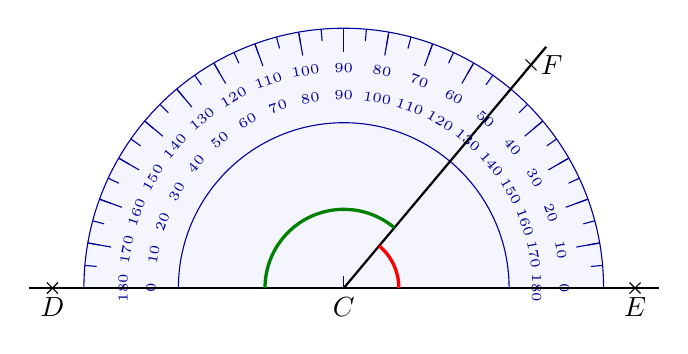
\begin{tikzpicture}[scale=1]
  \rapporteur
  \draw[thick] (-4,0) -- (4,0);
  \draw[thick] (0,0) -- (50:4);
  \croix{(3.7,0)} \node[below] at (3.7,0) {$E$};
  \croix{(-3.7,0)} \node[below] at (-3.7,0) {$D$};
  \croix{(50:3.7)} \node[right] at (50:3.7) {$F$};
  \node[below] at (0,0) {$C$};
  \draw[red, very thick] (0:0.7) arc[start angle=0, end angle=50, radius=0.7];
  \draw[green!50!black, very thick] (50:1) arc[start angle=50, end angle=180, radius=1];
\end{tikzpicture}
\end{minipage}\hfill
\begin{minipage}[c]{0.43\linewidth}
\textbf{Méthode :} je place le \textbf{centre} du rapporteur sur le sommet $C$,
et le \textbf{0} sur un côté.
\begin{itemize}[label=\textbullet]
\item Pour $\textcolor{red}{\widehat{FCE}}$, le côté $[CE)$ est sur le 0 de la graduation \textbf{extérieure} :
je lis $\widehat{FCE} = 50\degre$.
\item Pour $\textcolor{green!50!black}{\widehat{FCD}}$, le côté $[CD)$ est sur le 0 de la graduation \textbf{intérieure} :
je lis $\widehat{FCD} = 130\degre$.
\end{itemize}
\textit{Je vérifie :} $\widehat{FCE}$ est aigu, donc moins de $90\degre$.
\end{minipage}
\end{center}

\begin{notation}
Deux angles de même mesure sont codés de la même façon : ici $\widehat{IHJ} = \widehat{KML}$.
\end{notation}
\vspace{-4mm}
\begin{center}
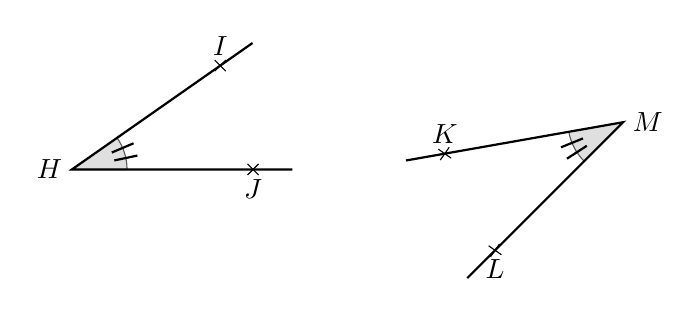
\begin{tikzpicture}
  \begin{scope}
    \draw[gray!70!black, fill=gray!25] (0,0) -- (7mm,0) arc[start angle=0, delta angle=35, radius=7mm] -- cycle;
    \draw[thick] (12:5.5mm) -- (12:8.5mm) (23:5.5mm) -- (23:8.5mm);
    \draw[thick] (2.8,0) -- (0,0) -- (35:2.8);
    \croix{(2.3,0)} \croix{(35:2.3)}
    \node[left] at (0,0) {$H$}; \node[below] at (2.3,0) {$J$}; \node[above] at (35:2.3) {$I$};
  \end{scope}
  \begin{scope}[shift={(7,0.6)}, rotate=190]
    \draw[gray!70!black, fill=gray!25] (0,0) -- (7mm,0) arc[start angle=0, delta angle=35, radius=7mm] -- cycle;
    \draw[thick] (12:5.5mm) -- (12:8.5mm) (23:5.5mm) -- (23:8.5mm);
    \draw[thick] (2.8,0) -- (0,0) -- (35:2.8);
    \croix{(2.3,0)} \croix{(35:2.3)}
    \node[right] at (0,0) {$M$}; \node[above] at (2.3,0) {$K$}; \node[below] at (35:2.3) {$L$};
  \end{scope}
\end{tikzpicture}
\end{center}

\begin{remarque}
Rappel (partie 2) : \textbf{l'angle droit} mesure $90\degre$
et \textbf{l'angle plat} mesure $180\degre$.
\end{remarque}

\newpage
\section{Construire un angle}
\comp{6C04-GEO15/16}{construire un angle de mesure donnée}

\textbf{Énoncé :} Tracer un angle $\widehat{BAC}$ de mesure $137\degre$.

\newcommand{\etapeConstr}[2]{%
\par\medskip\noindent
\begin{minipage}[c]{0.4\linewidth}#1\end{minipage}\hfill
\begin{minipage}[c]{0.58\linewidth}\centering
\begin{tikzpicture}[scale=0.92]
  \useasboundingbox (-4.6,-0.6) rectangle (4.3,3.8);
  #2
  \draw[thick] (0,0) -- (4.2,0);
  \croix{(3.8,0)} \node[below] at (3.8,0) {$B$};
  \node[below] at (0,0) {$A$};
\end{tikzpicture}
\end{minipage}\par}

\etapeConstr{\textbf{Étape 1 :} je trace la demi-droite $[AB)$. Je place le \textbf{centre} du rapporteur sur $A$
et le \textbf{0} sur $[AB)$.}{\rapporteur}

\etapeConstr{\textbf{Étape 2 :} le 0 posé sur $[AB)$ est celui de la graduation \textbf{extérieure}.
Je cherche $137$ sur la graduation extérieure et je fais une \textbf{marque} au crayon.}
{\rapporteur \draw[red, thick] (137:3.45) ++(-3pt,-3pt) -- ++(6pt,6pt) ++(-6pt,0) -- ++(6pt,-6pt);
 \node[red, left] at (137:3.55) {marque};}

\etapeConstr{\textbf{Étape 3 :} je retire le rapporteur. Je trace la demi-droite d'origine $A$ qui passe par la marque,
et je place un point $C$ dessus. Je code l'angle.}
{\draw[gray!70!black, fill=gray!25] (0,0) -- (6mm,0) arc[start angle=0, delta angle=137, radius=6mm] -- cycle;
 \draw[thick] (0,0) -- (137:4);
 \draw[red, thick] (137:3.45) ++(-3pt,-3pt) -- ++(6pt,6pt) ++(-6pt,0) -- ++(6pt,-6pt);
 \croix{(137:2.6)} \node[below left] at (137:2.6) {$C$};
 \node at (68.5:1.1) {$137\degre$};}

\end{document}
